\section{Design Language}
\label{design:design_language}

\subsection{Status icons}
\label{design:state_icons}

In the \giraf[] system there are different status icons for showing the user what an action will do or is doing. All these icons can be seen in \autoref{fig:status_icons}. If an action accepts the leftmost icon will be used and if a window is loading the fourth leftmost icon will be shown maybe with an animation so that the user knows for sure that the window is not crashed.

\begin{figure}[h!]
	\centering
	
\includegraphics[width=\textwidth]{gfx/status_icons}
	\caption{Status icons in the \giraf[] system}
	\label{fig:status_icons}
\end{figure}

The icons in \autoref{fig:status_icons} includes: Accept, reject, synchronizing, loading and not found, seen from the left.

\subsection{Colors}
\label{design:giraf_colors}

Colors where chosen for the \giraf[] system these can be seen in \autoref{fig:colortheme}. These colors is designed for use in two different cases. The first four yellow and brown colors is made for use together and the last four colors white and grey is made for use together. These color groups is chosen such that they have contrast and can make gradients.

\begin{figure}[h!]
	\centering
	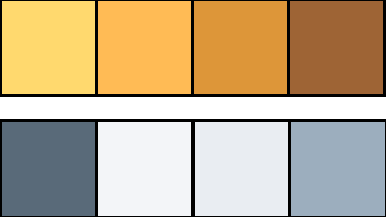
\includegraphics[width=\textwidth]{gfx/design_color_theme}
	\caption{The color theme of the \giraf[] system}
	\label{fig:colortheme}
\end{figure}

\subsection{Interactive elements}
\label{design:button_design}

In the \giraf[] system all interactive elements should have round corners. This was decided to make the overall consistency and usability in the \giraf[] system better this was done because of \autoref{Preanalysis:Usability_for_children}, where it states that recognition is better.
If an element is not interactive they should have square corners.
These guidelines also includes colors of buttons. All buttons should have the brown color on all sides and the middle should be yellow.

This section will use buttons as an example of an interactive element but the interactive elements in the \giraf[] system also includes dragable objects and other touch objects. The example can be seen in \autoref{fig:buttons}

\begin{figure}[h!]
	\centering
	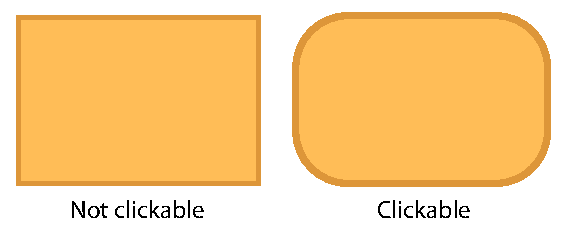
\includegraphics[width=\textwidth]{gfx/buttons.pdf}
	\caption{Interactive elements: Buttons illustrations}
	\label{fig:buttons}
\end{figure}